\documentclass[crop,tikz]{standalone}
\usetikzlibrary{backgrounds}
\colorlet{blue}{cyan}
\tikzset{
  inverted/.style = {
    color=white,
    background rectangle/.style={fill},
    show background rectangle
  }
}
\usepackage{pgfplots}
\pgfplotsset{compat=1.13}

% Lines of constant potential for a cylinder of radius 1/4 at position
% z = 1/2 inside a 2nd cylinder of radius 1 at position z = 0.
%
% Inspired by the expressions given Arens, chapter 32.2.

\pgfplotsset{
  inverted/.style = {
    every axis legend/.append style={
      draw=white,
      fill=black,
      text=white
    }
  },
  every non boxed x axis/.append style={
    axis line style={-latex}
  },
  every non boxed y axis/.append style={
    axis line style={-latex}
  }
}

\begin{document}

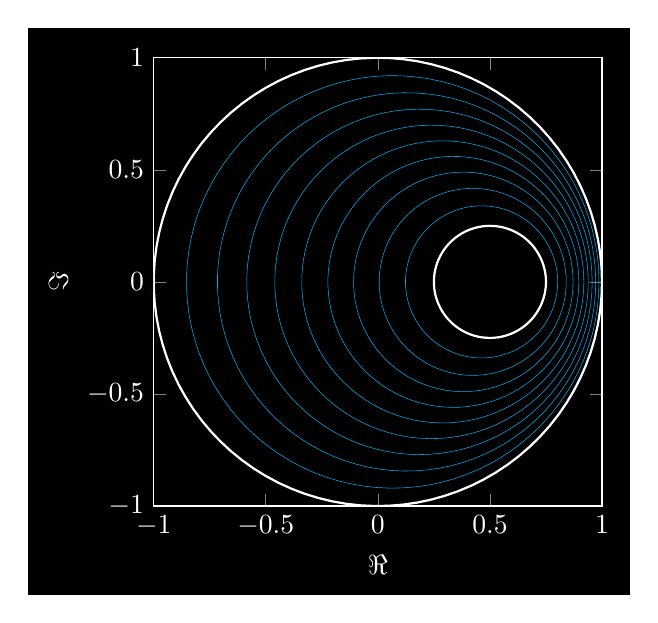
\begin{tikzpicture}[inverted,inverted]
  \pgfmathsetmacro{\numberofpotentiallines}{10};
  \pgfmathsetmacro{\zo}{(19 - sqrt(105))/16};
  \pgfmathsetmacro{\rmin}{1/4}; % radius of inner cylinder
  \pgfmathsetmacro{\rmax}{1}; % radius of outer cylinder
  \pgfmathsetmacro{\remin}{-1};
  \pgfmathsetmacro{\remax}{-\remin};
  \pgfmathsetmacro{\immin}{-1};
  \pgfmathsetmacro{\immax}{-\immin};
  \begin{axis}[inverted,
    axis equal image,
    xmin={\remin}, xmax={\remax},
    ymin={\immin}, ymax={\immax},
    xlabel={$\Re$},
    ylabel={$\Im$},
    samples=100,
    domain=0:360,
    declare function = {
      phixo(\c,\zo) = \zo*(1 - \c)/(1 - \c*\zo^2); % x-shift
      phir(\c,\zo) = sqrt(\c)*(1 - \zo^2)/(1 - \c*\zo^2); % radius
      phix(\x,\c,\zo) = phir(\c,\zo)*cos(\x) + phixo(\c,\zo);
      phiy(\x,\c,\zo) = phir(\c,\zo)*sin(\x);
      sqrtc(\r,\zo,\s) = -(1 - \zo^2)/(2*\r*\zo^2) + \s*sqrt(((1 - \zo^2)/(2*\r*\zo^2))^2 + 1/\zo^2); % sqrt(c) as a function of the radius r
      cmin(\zo) = sqrtc(\rmin,\zo,1)^2; % minimum c
      cmax(\zo) = sqrtc(\rmax,\zo,1)^2; % maximum c
      fc(\n,\nmax) = cmin(\zo) + \n/\nmax*(cmax(\zo) - cmin(\zo)); % calculates c
    },
    ]
    % lines of constant potential
    \pgfplotsinvokeforeach{0,...,{\numberofpotentiallines}}{
      \addplot[blue,very thin] (
        {phix(x, fc(#1,\numberofpotentiallines), \zo)},
        {phiy(x, fc(#1,\numberofpotentiallines), \zo)}
     );
    }
    % charges
    \addplot[thick] ({\rmax*cos(x)},{\rmax*sin(x)});
    \addplot[thick] ({\rmin*cos(x) + 0.5},{\rmin*sin(x)});
  \end{axis}
\end{tikzpicture}
\end{document}
